\section{Testing - Parameter Tuning} \label{actualTesting}
To begin my evaluative testing, I feel it necessary to tune the parameters of my algorithm that I believe impact its ability to generate good solutions. There are four key parameters:

\begin{itemize}
    \item \bf Number of Generations \rm - The number of times to run through the simulation game and create a new population. This number of generations occur every iteration. I anticipate that as this variable increases, the solution quality will increase. Eventually the payoff will begin to decrease as the algorithm starts overfitting.
    \item \bf Number of Iterations \rm - The number of segments to cut the data into. The first n-1 of these are used to train the algorithm, and the last is used to evaluate it. I'm not sure how this variable will affect payoff, but the generality of the screeners provided by the algorithm should improve as this variable increases.
    \item \bf Population Size \rm - The number of members of each population. Increasing this variable should increase the payoff.
    \item \bf Percentile Data Spread \rm - The gap between each percentile. This must be a number that divides 100 with no remainder. I'm not sure what impact this will have on payoff, but higher values of this variable will decrease the search space size. This is likely to impact the payoff in some way.
\end{itemize}

For each of these variables, I took four or more possible assignments to that variable - whilst keeping all of the other variables constant - and ran the algorithm with each assignment twenty times. I then looked at the best results from each of the twenty runs, and averaged them. The default values used for each variable are:
\begin{itemize}
    \item Number of Generations = 10
    \item Number of Iterations = 2
    \item Population Size = 100
    \item Percentile Data Spread = Gap of 10 between percentiles (10th, 20th, ..., 100th)
\end{itemize}

I would have conducted these tests over more than twenty runs of the algorithm, but due to the time that it takes to run the program, this was not feasible.

\vspace{30mm}

\begin{figure}[p]
    \setlength{\parindent}{24pt}
    \subsection{Number of Generations} \label{numGenTest}
    For these tests I used: 
    \begin{itemize}
        \item Number of Generations = \{2, 4, 6, 8, 10, 12, 14, 16, 18, 20\}
    \end{itemize}
    
    \begin{center}
        \pgfplotstabletypeset[
          columns/gen/.style={column name=Generations},
          columns/mean/.style={column name=Mean(\%)},
          columns/median/.style={column name=Median(\%)},
          columns/sd/.style={column name=Standard Deviation(\%)},
        ]{tables/generations-default.txt}
    \end{center}
    
    \noindent For the full tabular results see Appendix \ref{varyGen}.
    \vspace{4mm}
    
    {\centering
    \begin{tikzpicture}
        \begin{axis}[
            xlabel={Generations},
            ylabel={Payoff (\%)},
            legend pos=north east,
            legend entries={Mean,Median,SD},
        ]
        \addplot table [x=gen,y=mean] {tables/generations-default.txt};
        \addplot table [x=gen,y=median] {tables/generations-default.txt};
        \addplot table [x=gen,y=sd] {tables/generations-default.txt};
        \end{axis}
    \end{tikzpicture}}
    \newline
    
    These results are very mixed. We can see the expected drop off in mean and median payoff with a high number of generations, but this appears to be happening as low as 12 generations in. I anticipated that this would take far longer to occur. Also, the mean payoffs from 2 to 10 generations are largely the same. \newline

    I expected some increase in mean payoff with generation number early on in this test, but that has not happened. The median and standard deviation have acted as I expected. Additionally, I believe that the spike of poor results at generation 14 is an anomaly.
\end{figure}

\begin{figure}[p]
    \setlength{\parindent}{24pt}
    \subsection{Number of Iterations}
    For these tests I used:
    \begin{itemize}
        \item Number of Iterations = \{2,3,4,5\}
    \end{itemize}
    
    \begin{center}
        \pgfplotstabletypeset[
          columns/iter/.style={column name=Iterations},
          columns/mean/.style={column name=Mean(\%)},
          columns/median/.style={column name=Median(\%)},
          columns/sd/.style={column name=S.D.(\%)},
        ]{tables/iterations-default.txt}
    \end{center}
    
    \noindent For the full tabular results see Appendix \ref{varyIter}.
    \vspace{4mm}
    
    {\centering
    \begin{tikzpicture}
        \begin{axis}[
            xlabel={Iterations},
            ylabel={Payoff (\%)},
            legend pos=north east,
            legend entries={Mean,Median,S.D.},
        ]
        \addplot table [x=iter,y=mean] {tables/iterations-default.txt};
        \addplot table [x=iter,y=median] {tables/iterations-default.txt};
        \addplot table [x=iter,y=sd] {tables/iterations-default.txt};
        \end{axis}
    \end{tikzpicture}}
    \newline
    
    These results are not at all what I was expecting. Each iteration uses a separate set of data to train on, so by adding further iterations, the algorithm protects against overfitting. As the number of iterations increases, the generalisation of the screening strategies that the algorithm produces should increase. This is due to the algorithm having less chance to memorise training data, instead of learning its patterns. \newline
    
    My interpretation as to why more than two iterations negatively impacts payoff, is that by using more iterations the algorithm is being given the opportunity to ``forget'' what it learned in earlier iterations. When all of the data to be trained on is used in one iteration, every piece of information has been seen more recently and so can impact the resulting screening strategy. \newline
    
    When more iterations are added, the pieces of information seen in the first iteration are  now further away in time. Consider the following analogy involving a student and a teacher.
    
\end{figure}

The teacher has a set of d problems for the student to complete. They are split into k sets, where each set of problems must be fully completed G times before moving on. The first k-1 sets are done for the student to learn, with the last being for the teacher to evaluate the students performance. This is exactly how my algorithm behaves; the student represents the solutions, the teacher represents the algorithm. \newline

\hspace{-18pt} 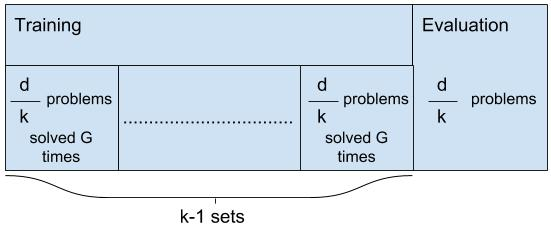
\includegraphics[width=\textwidth]{images/drawing-analogy.jpg}

\hspace{-18pt} 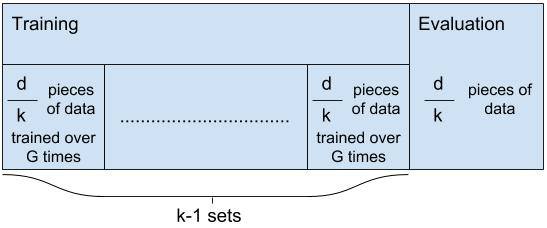
\includegraphics[width=\textwidth]{images/drawing-system.jpg}

\begin{itemize}
    \item When k = 2, the first problem in the first set is last completed 
    \begin{equation}
        \frac{d}{2}
    \end{equation}
    training problems ago when the algorithm finishes training.
    \item When k = 3, the first problem in the first set is last completed 
    \begin{equation}
       \frac{d}{3} + \frac{d}{3}G = \frac{d}{3}(G + 1)
    \end{equation}
    training problems ago when the algorithm finishes training.
    \vspace{20mm}
    \item When k = n, the first problem in the first set is last completed
    \begin{equation}
        \frac{d}{n} + \frac{d}{n}G(n-2) = \frac{d}{n}(G(n - 2) + 1)
    \end{equation}
    training problems ago when the algorithm finishes training.
\end{itemize}
  By dividing the k = n case by the k = 2 case, we can work out how many more problems (as a ratio) have been solved in the k = n case, since the first problem in the first set was last solved:

\begin{equation}
    \frac{\frac{d}{n}(G(n - 2) + 1)}{\frac{d}{2}} = 2G + \frac{2-4G}{n}
\end{equation}

So, there is $2G + \frac{2-4G}{n}$ times more learning to be done after the first piece of training data is last seen. I suggest that this implies that the algorithm will bias towards the most recent set of training data, effectively forgetting the iterations over the sets of training data before it.

\clearpage

\begin{figure}[p]
    \setlength{\parindent}{24pt}
    \subsection{Population Size}
    For these tests I used:
    \begin{itemize}
        \item Population Size = \{50,75,100,125,150,175\}
    \end{itemize}
    
    \begin{center}
        \pgfplotstabletypeset[
          columns/lambda/.style={column name=Population Size},
          columns/mean/.style={column name=Mean(\%)},
          columns/median/.style={column name=Median(\%)},
          columns/sd/.style={column name=S.D.(\%)},
        ]{tables/lambda-default.txt}
    \end{center}
    
    \noindent For the full tabular results see Appendix \ref{varyLambda}.
    \vspace{4mm}

    {\centering
    \begin{tikzpicture}
        \begin{axis}[
            xlabel={Population Size},
            ylabel={Payoff (\%)},
            legend pos=south east,
            legend entries={Mean,Median,S.D.},
        ]
        \addplot table [x=lambda,y=mean] {tables/lambda-default.txt};
        \addplot table [x=lambda,y=median] {tables/lambda-default.txt};
        \addplot table [x=lambda,y=sd] {tables/lambda-default.txt};
        \end{axis}
    \end{tikzpicture}}
    \newline
    
    These results are, largely, as I expected. It is generally accepted that increasing the population size in any genetic algorithm will improve its results. This is because a larger population allows the algorithm to explore more of the search space. This has diminishing returns with large populations, as increasing the population size will also increase the time that the algorithm takes. \newline
    
    My results agree with this, except for population sizes 125 and 150. As all of these experiments are heavily influenced by the initialisation of the algorithm, I anticipate that if I repeated this experiment with 40 runs instead of 20, these points would be closer to the results for 100 or 175. \newline
    
    As such, I am happy to conclude that higher population sizes improve the solution quality.
\end{figure}

\begin{figure}[p]
    \setlength{\parindent}{24pt}
    \subsection{Percentile Data Spread}
    For these tests I used:
    \begin{itemize}
        \item Percentile Data Spread = Gaps of \{1, 2, 4, 5, 10\} between percentiles
    \end{itemize}
    
    \begin{center}
        \pgfplotstabletypeset[
          columns/perc/.style={column name=Percentile Gap},
          columns/mean/.style={column name=Mean(\%)},
          columns/median/.style={column name=Median(\%)},
          columns/sd/.style={column name=Standard Deviation(\%)},
        ]{tables/percentiles-default.txt}
    \end{center}
    
    \noindent For the full tabular results see Appendix \ref{varyPerc}.
    \vspace{4mm}
    
    {\centering
    \begin{tikzpicture}
        \begin{axis}[
            xlabel={Percentile Gap},
            ylabel={Payoff (\%)},
            legend pos=north east,
            legend entries={Mean,Median,S.D.},
        ]
        \addplot table [x=perc,y=mean] {tables/percentiles-default.txt};
        \addplot table [x=perc,y=median] {tables/percentiles-default.txt};
        \addplot table [x=perc,y=sd] {tables/percentiles-default.txt};
        \end{axis}
    \end{tikzpicture}}
    \newline
    
    Standard Deviation stays relatively constant across all five assignments, whilst mean and median are maximised at gaps of 2 and 5, and perform substantially worse at 1, 4, and 10. \newline
    
    I am not sure why a gap size of 4 performs so much worse than 2 or 5. It could be an anomaly, but I am unwilling to come to that conclusion on such a small sample size.
    
\end{figure}

\begin{figure}
    \subsection{Summary of Tests}
    \begin{itemize}
        \item Increasing the number of generations per iteration reduces solution quality after around 12 generations. I am going to use 12 as my default number of generations, as it had the best median result and the third best mean result.
        \item Increasing the number of iterations dramatically reduces solution quality. Two iterations is always the best option.
        \item Increasing population size improves solution quality. As a trade off for time, I am going to use a population size of 150.
        \item Changing the number of percentiles does not consistently change solution quality. I am going to use a percentile gap of 2, as it had the best median result, the second best mean result, and a slightly lower standard deviation.
        \item The standard deviations calculated across all four tests are remarkably high. Looking at the profits in the full results tables in Appendices \ref{varyGen}-\ref{varyPerc}, there is a large variance in solution quality from run to run. This would imply that the initialisation of the algorithm is very important in deciding whether the screeners it produces will be good. This is likely due to the size of the search space, and my current lack of niching operators.
    \end{itemize}
    
    \subsection{Suggested Further Changes}
    Following the observation I made about standard deviation above, I intend to experiment with adding elitism during population generation, as well as a speciation method during selection. \newline
    
    One of the possible reasons for the standard deviation being so high, is that the algorithm is losing good solutions. This could be due to:
    \begin{itemize}
        \item \bf Random Chance \rm - These solutions are simply not being selected or are being mutated away.
        \item \bf Poor Crossover \rm - The solutions are irreparably damaged when they are crossed with another solution during the crossover function.
    \end{itemize}
    
    An elitism approach protects against both of these. \newline
    
    Another possibility is that the algorithm is simply not able to search the space as effectively as it needs to. The must likely reason for this is premature convergence of candidate solutions. A speciation method would force diversity within the population, meaning more of the search space can be explored.
    
\end{figure}